\documentclass[a4paper]{article}

\usepackage[english]{babel}
\usepackage[utf8x]{inputenc}
\usepackage{amsmath}
\usepackage{amsfonts}
\usepackage{graphicx}
\usepackage[colorinlistoftodos]{todonotes}

\title{CS 5785 -- Applied Machine Learning -- Lec.\ 9}
\author{Prof.\ Nathan Kallus, Cornell Tech\\Scribe: TBD}
\date{Sept.\ 21, 2017}

\begin{document}
\maketitle

\section{Kernel Density Estimation}

During this course we use the term \textit{kernel} in two separate ways:
\begin{enumerate}
\item A device for local weighted averaging, related to the use of kernels in convolution.
\item A generalization of an inner product for non-linear machine learning.
\end{enumerate}
This lecture focuses on the first kind of kernel.  In the last lecture we saw the application of kernels to the problem of smoothing a noisy function.  Now we will study the related problem of \emph{Kernel Density Estimation}, which we can think of as a continuous counterpart to a histogram.  Where a histogram requires us to define the \emph{bin width}, in kernel density estimation we must define the \emph{kernel width}. Later, we'll learn that Kernel Density is used as an estimate probability distribution function.


Suppose we have a random sample $x_1, \ldots, x_N$ drawn from pdf (probability density function) $f_X(x)$ (assuming $X\in \mathbb{R}$) and we want to estimate $f_X$ at a new point $x_0$. Before appealing to kernels, a very simple approach for computing this estimate $\hat{f}_X(x_0)$ would be to use a simple average of the samples within a small neighborhood around $x_0$ of width $\lambda$. This is called \textit{neighbor-based density esimation}:
$$\hat{f}_X(x_0)=\frac{\#x_i \in \mathcal{N}(x_0)}{N\lambda}$$
In analogy to the $k$-NN based smoothing approach from last lecture, this method will produce a jumpy estimate of the density: if we imagine sliding the neighborhood along the horizontal axis, samples will pop in and out of the averaging interval discontinuously, causing corresponding fluctuations in $\hat{f}_X$.


\subsection{Parzen Estimate}
The kernel smoothing counterpart to the above method is expressed as follows:
$$\hat{f}_X(x_0)=\frac{1}{N\lambda}\sum_{i=1}^N K_\lambda(x_0, x_i)$$
Where $K_\lambda(x_0, x)=\phi(|x-x_0|/\lambda)$ is the kernel of width $\lambda$ centered around $x_0$ at a point $x$. This is also known as a \emph{Parzen estimate} and choices of kernels such as a Gaussian or triangle are known as \emph{Parzen windows}.  An example of kernel density estimation using a Gaussian is shown in Figure \ref{fig:Figure613}.

\begin{figure}
\centering
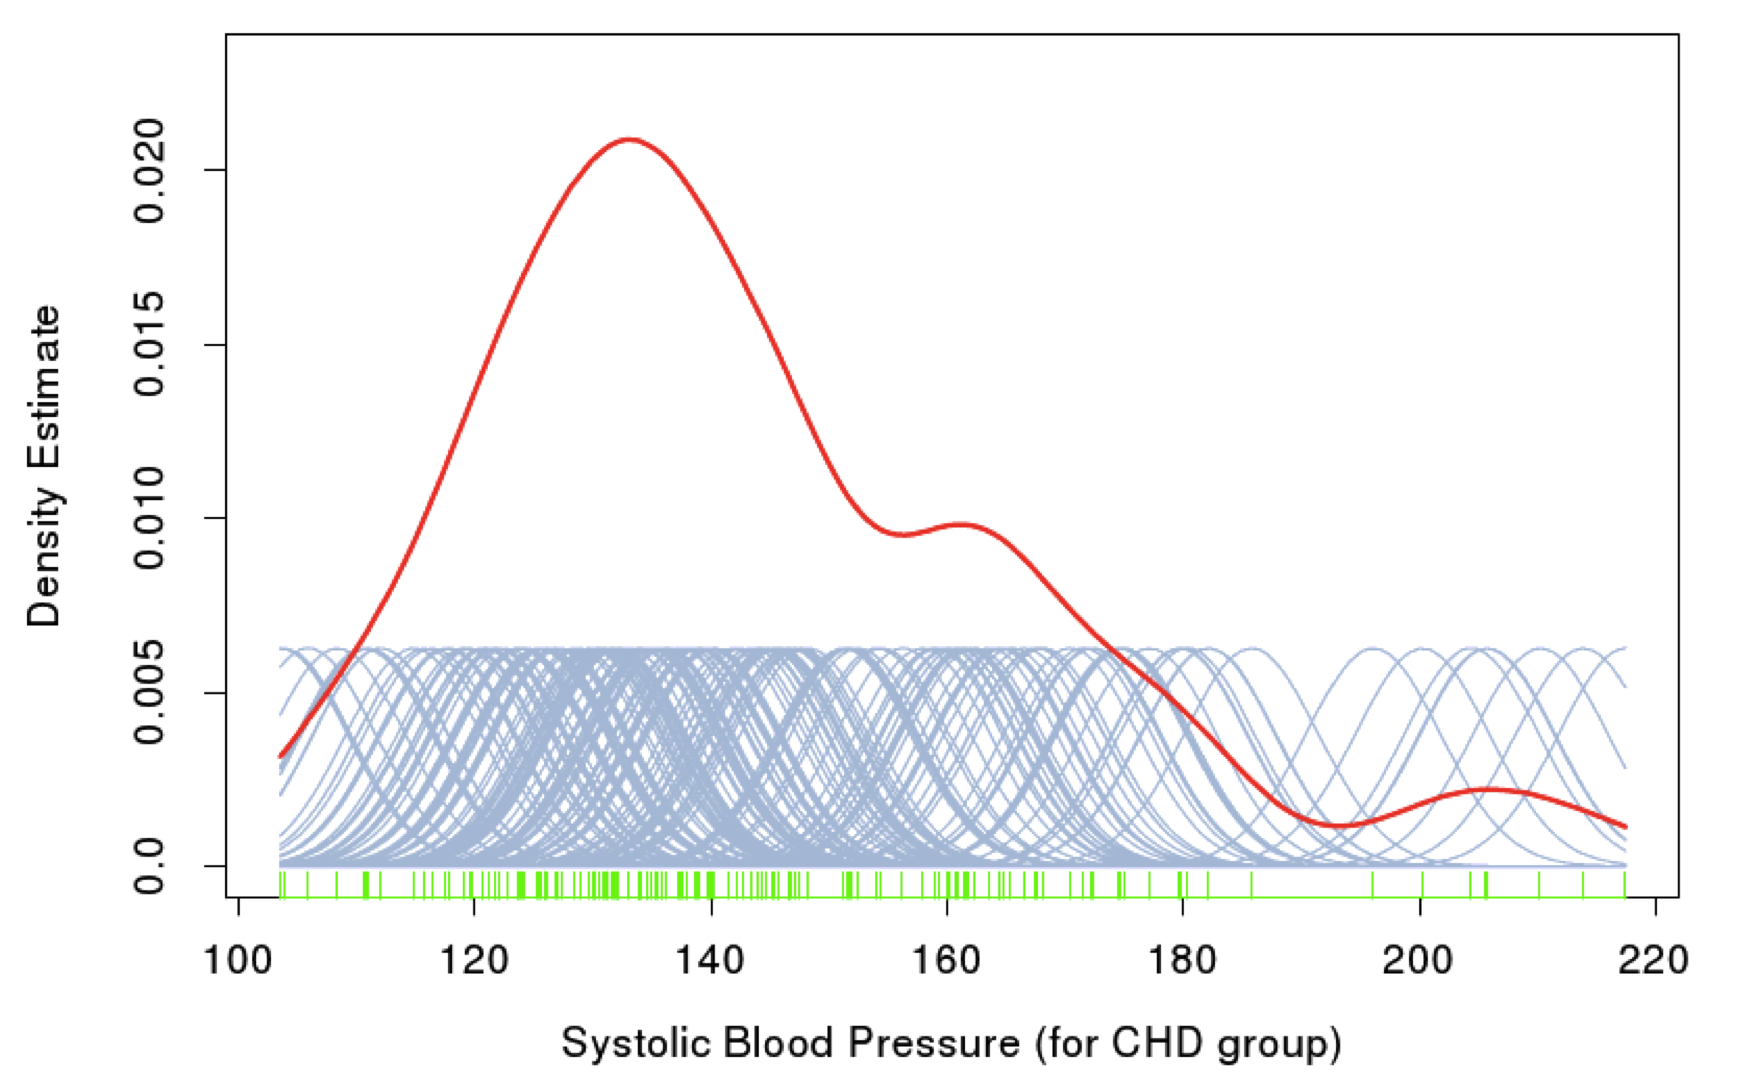
\includegraphics[width=1.0\textwidth]{Figure613.png}
\caption{\label{fig:Figure613}[HTF Figure 6.13] Each green tick represents a single recorded observation. Each tick, which we can think of as a unit impulse function, is replaced with a kernel function -- a Gaussian in this case -- represented by the blue curves.  The kernel density estimate, shown in red, is simply the sum of all these kernels. The red figure adds up all Gaussians and thus there's a bugger bump where the Gaussians are more crowded. As a side note, in order to choose the right width of the Gaussians we need to use cross-validation. (CHD=Congenital Heart Disease)}
\end{figure}

The Parzen Estimate is closely related to convolution:
$$\hat{f}_X(x)=\frac{1}{N}\sum_{i=1}^N \phi_\lambda(x-x_i)= (\hat F * \phi_\lambda )(x)$$
where $\phi_\lambda(\cdot)$ is a Gaussian density and $\hat F$ is an impulsive distribution with mass of $1/N$ at each $x_i$.  
This is equivalent to adding iid Gaussian noise to each observation $x_i$.\footnote{See ``convolution of probability distributions'' on Wikipedia.}
%\footnote{See \url{http://en.wikipedia.org/wiki/Convolution_of_probability_distributions}}
As in the case of bin width selection for histograms, the choice of kernel width can dramatically impact the appearance of the density estimate; see Figure \ref{fig:KernelWidth}.  When applying KDE on supervised learning problems, one can use cross validation to choose the best kernel width $\lambda$.

\begin{figure}
\centering
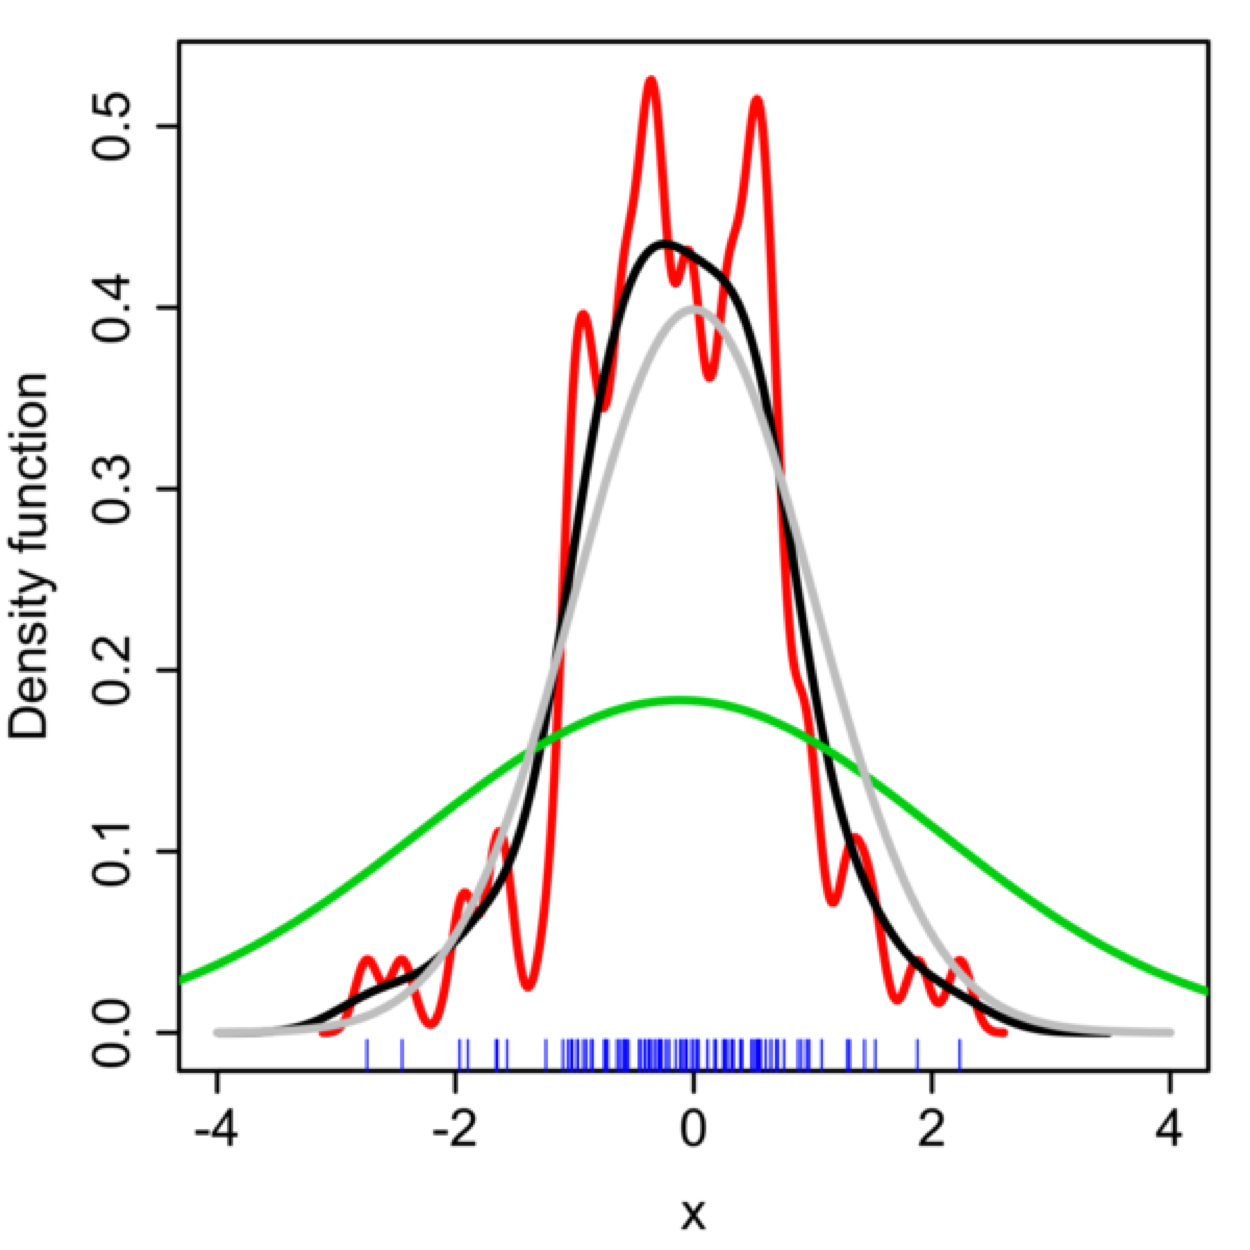
\includegraphics[width=0.5\textwidth]{KernelWidthSelection.png}
\caption{\label{fig:KernelWidth}Kernel density estimate (KDE) with different bandwidths of a random sample of 100 points from a standard normal distribution. Grey: true density (standard normal). Red: KDE with $\lambda=0.05$. Green: KDE with $\lambda=2$. Black: KDE with $\lambda=0.337$. [Wikipedia]}
\end{figure}

\subsection{KDE based Classification}

Suppose we have a $J$ class problem. Fit a KDE $\hat{f}_j(x)$, $j = 1, \ldots, J$ separately for each class and estimate the priors $\hat{\pi}_j$ using the sample proportions. Bayes' rule tells us that the resulting posterior is: 
$$\hat{Pr}(G=j | X=x_0)=\frac{\hat{\pi}_j \hat{f}_j (x_0)}{\sum_{k=1}^J \hat{\pi}_k \hat{f}_k (x_0)}$$
The classifier returns the class $j \in G$ with the highest posterior probability.

\begin{figure}
\centering
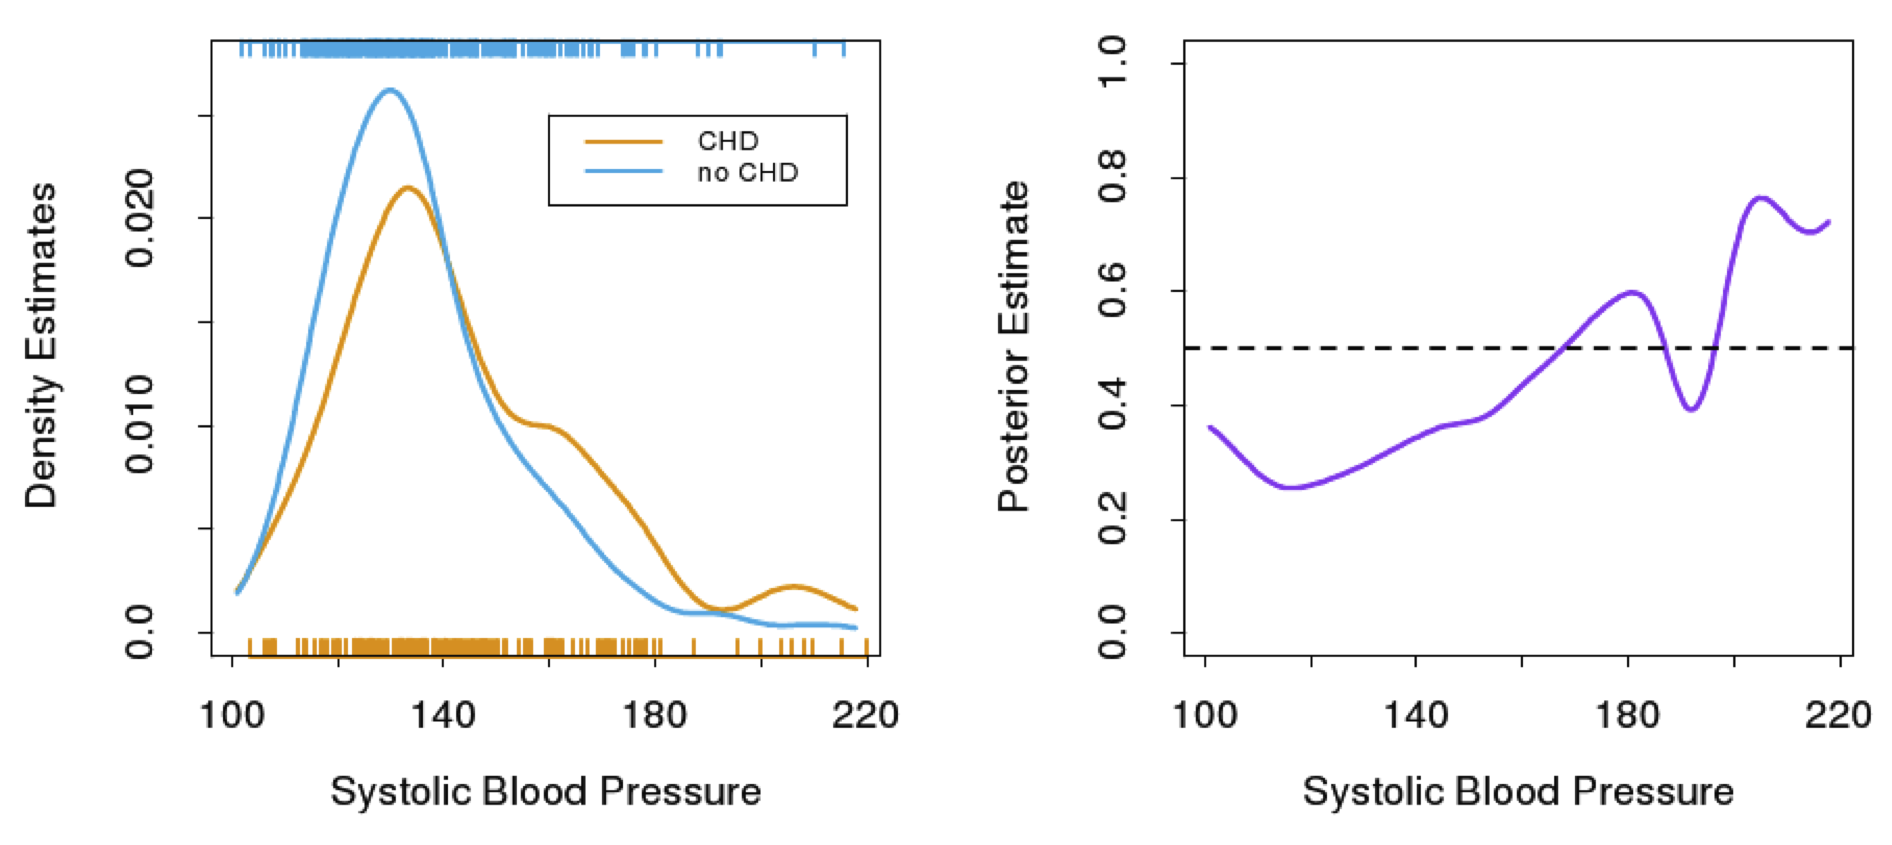
\includegraphics[width=1.0\textwidth]{Figure614.png}
\caption{\label{fig:Figure614}[HTF Figure 6.14] The left graph shows the KDEs for 2 classes and the right graph shows the classification result (where the dashed line represents the decision threshold).}
\end{figure}

In Figure \ref{fig:Figure614} we see how based on the KDE in a 2 class scenario we get a threshold that separates the two classes. The fluctuating, wiggly behavior around 190-200 mm Hg arises from the sparsity of the data in that section.  Very few points fall inside the kernel there and the expression for the posterior becomes unstable; as if it were ``hallucinating'' data.
One way to address this, which we won't be covering, is to use a kernel with adaptive width.




\subsubsection{Discriminative vs. Generative}

\begin{figure}
\centering
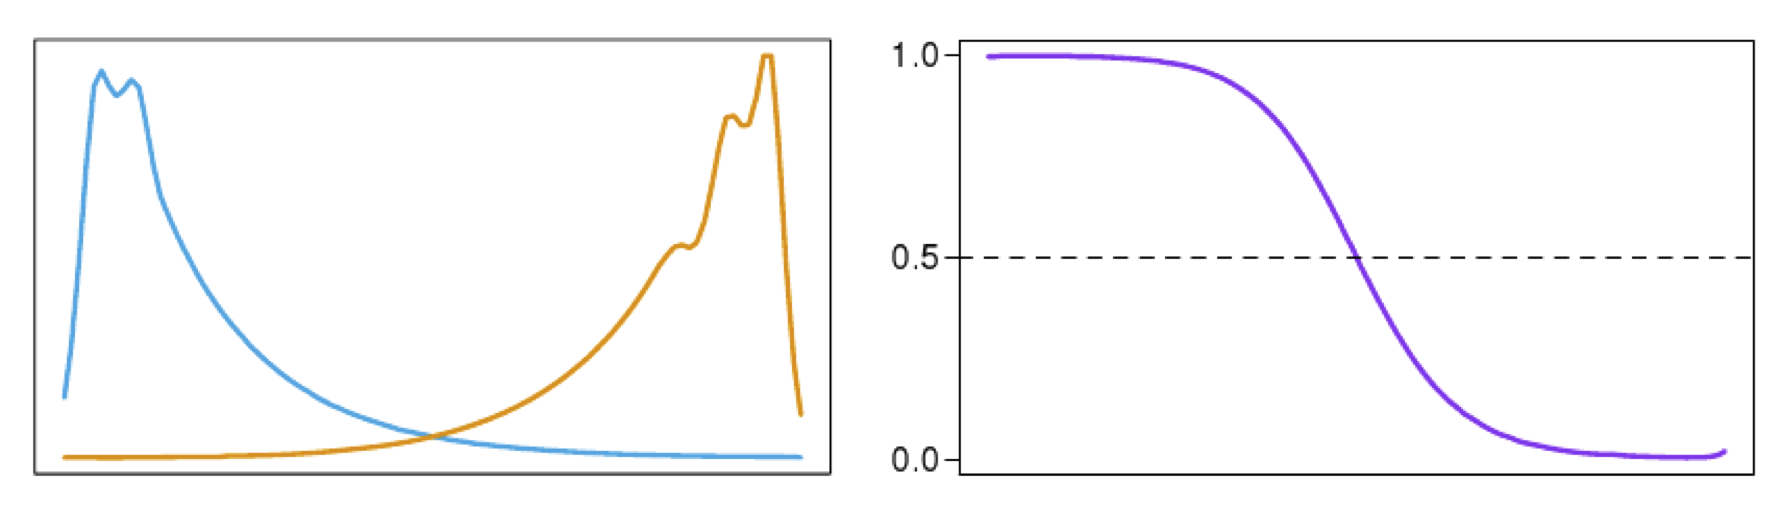
\includegraphics[width=1.0\textwidth]{Figure615.png}
\caption{\label{fig:Figure615}[HTF Figure 6.15] The population class densities may have interesting structure (left) that disappears when the posterior probabilities are formed (right). The dashed line in the right depicts the threshold.}
\end{figure}

In Figure \ref{fig:Figure615} the left graph shows two class densities
and the right graph shows the posterior probability.  It's worth reflecting on the fact that some potentially interesting structure in the class densities is lost in this operation.  If all we care about is separating the class, i.e. if we take a \emph{discriminative} viewpoint, we needn't worry; clearly a threshold of 0.5 will do a good job of separating the classes, and we in fact only need to put effort into estimating the posterior near the decision boundary.  If we're also interested in characterizing the individual class densities, e.g., for synthesizing realistic data for simulations, we may prefer the \emph{generative} viewpoint, for which careful modeling of the multimodal bumps in the two densities would play an important role in the characterizations. Generative algorithms model how data was generated for  classification while discriminitive algorithms do not care how it was generated.


\subsection{The Curse of Dimensionality}
All the examples we have seen in this lecture so far were 1 dimensional.  In the blood pressure example, we saw that sparsity created a problem, i.e., there weren't enough data points to provide a reliable KDE in a certain subinterval.  Similarly, if we were histogramming, we'd have some bins with few or no point counts.  When we scale up to higher dimensions empty bins become much more common.  When we divide a 1D bin into 10 bins we get 10 bins, but when we divide a 3D bin with the same granularity along each dimension we get 1000 bins.  This problem is one manifestation of the \textit{curse of dimensionality} (Bellman, 1961).

\section{Naive Bayes}
A very popular and surprisingly effective way to deal with the curse of dimensionality when dealing with a high dimensional classification problem (where $p\gg 1$) is \textit{Naive Bayes}.\\
Naive Bayes assumes that given a class $G=j$, the feature vectors $x_k$ are independent (hence the "naive" in the name) and ignores the joint probabilities.$$f_j(X)=\prod_{k=1}^p f_{jk}(X_k)$$
This is a very simple case of a generative model.  Obviously, this assumption is not very realistic, but it tends to do reasonable things at the class boundary. The consequences of this simplification are as follows:
\begin{itemize}
\item Individual class conditional marginal density $f_{j_k}$ can each be estimated using a 1D kernel density estimate.
\item If some component $X_j$ is discrete, no problem, we can swap in a histogram for its density estimate.
\end{itemize}
Naive Bayes handles curse of dimensionality by putting each feature in its own "silo". With its focus on the behavior near the decision boundary, Naive Bayes often performs better than far more sophisticated alternatives.

The log-odds transformation in this case (using class $J$ as the base) is given by:
$$\log \frac{Pr(G=l|X)}{Pr(G=J|X)}=\log \frac{\pi_l f_l (X)}{\pi_J f_J (X)}=\log \frac{\pi_l \prod_{k=1}^p f_{lk}(X_k)}{\pi_J \prod_{k=1}^p f_{Jk}(X_k)}$$
$$\Downarrow$$
$$\log \frac{Pr(G=l|X)}{Pr(G=J|X)}=\log \frac{\pi_l}{\pi_J} + \sum_{k=1}^p \log \frac{f_{lk}(X_k)}{f_{Jk}(X_k)}$$
If we let $\log \frac{f_{lk}(X_k)}{f_{Jk}(X_k)}=g_{lk}(x_k)$ and $\frac{\pi_l}{\pi_J}=\alpha_l$ we get:
$$\log \frac{Pr(G=l|X)}{Pr(G=J|X)}=\alpha_l + \sum_{k=1}^p g_{lk}(x_k)$$
Incidentally this has the same form as the ``generalized additive model'' but it is fit differently.  This is analogous to Logistic Regression and Linear Discriminant Analysis having the same functional form but different modeling assumptions and fitting procedures. Note that $g_{l_k}$ in the above equation is a nonlinear function. 


\end{document}
